\begin{problem}{이름 궁합}
{}{}
{1초}{512MB}{}

\textit{`이름 궁합'}이란 두 사람의 이름을 한 글자씩 번갈아 써 놓고 획수를 그 아래에 적은 뒤, 인접한 숫자끼리 더한 일의 자리 값을 아래에 적어 나가면서 마지막에 남은 두 숫자를 보고 궁합이 맞는 정도를 알아보는 일종의 점이다.

아직도 \textit{`그녀'}를 잊지 못한 로맨티스트 종민이는 어느 날 그녀와 이름 궁합을 한 번 해 보기로 했는데, 그 결과는 충격적이었다.

\begin{figure}[h]
	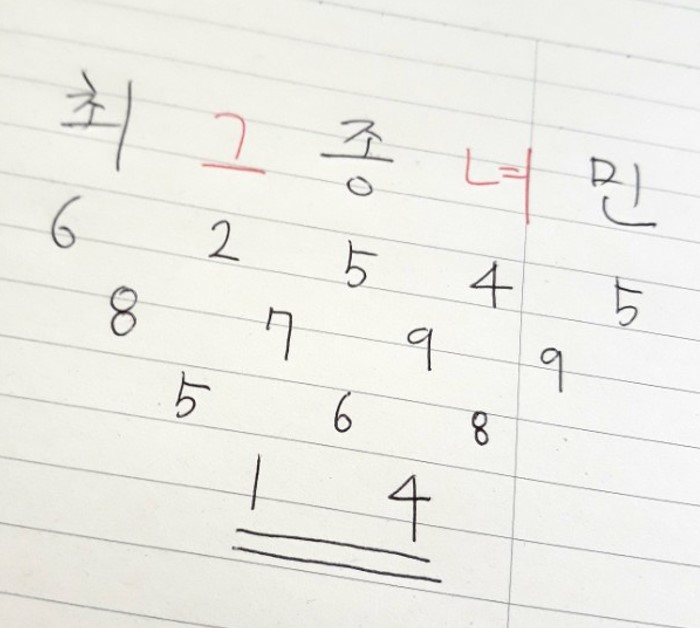
\includegraphics[width=8cm]{./problems/H_namechemi_1.jpg}
	\centering
\end{figure}

이 결과를 도저히 받아들일 수 없었던 종민이는 이것이 틀렸음을 증명하기 위해 열심히 머리를 굴렸고, 다음과 같은 변명거리를 생각해 냈다.

\textit{```그녀'는 한국인이 아니니까 한글로 이름 궁합을 보면 결과가 이상한 것이 당연하지! 세계 공용어인 영어 알파벳으로 이름을 쓰면 결과가 정확하게 나올 거야!''}

그래서 종민이는 알파벳 대문자로 이름을 써 놓고 이름 궁합을 보려고 한다. 그런데, 종민이는 손으로 계산을 하면 실수를 할까 두려워 당신에게 프로그램을 짜 달라고 부탁했다. 종민이를 도와주자!
종민이가 정한 알파벳 대문자의 획수는 \textbf{Note}를 참고하자.

\InputFile

첫 번째 줄에는 종민이의 영어 이름 $A$가 주어진다. 

두 번째 줄에는 `그녀'의 영어 이름 $B$가 주어진다.

$A$와 $B$ 모두 알파벳 대문자로만 이루어진 길이 $2$ 이상 $2\, 000$ 이하의 문자열이며, 둘의 길이가 같음이 보장된다. 이름 궁합을 볼 때는 $A$의 첫 글자를 먼저 쓴다고 하자.

\OutputFile

이름 궁합의 결과를 두 자리의 숫자로 출력한다. (십의 자리가 0이어도 두 자리로 출력한다)

\Examples
	
\begin{example}
\exmp{
CJM
HER
}{%
99
}%
\end{example} 

\Note

영어 대문자 알파벳 26개의 획수는 순서대로 3, 2, 1, 2, 3, 3, 2, 3, 3, 2, 2, 1, 2, 2, 1, 2, 2, 2, 1, 2, 1, 1, 1, 2, 2, 1 로 정한다.\footnote{출제자가 알파벳 대문자를 쓰는 방법이 기준이다}

\end{problem}
